% file: 3-7-sssp/dijkstra-correctness.tex

\documentclass[tikz]{standalone}
\usetikzlibrary{shapes, positioning, decorations.pathmorphing, backgrounds, fit}

\begin{document}
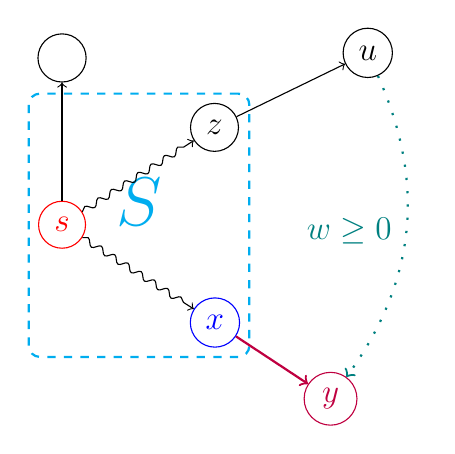
\begin{tikzpicture}[every node/.style = {draw, circle, minimum size = 8pt, font = \large},
  node distance = 0.8cm and 1.5cm,
  every edge/.style = {draw, ->},
  path/.style = {->, decorate, decoration = {snake, amplitude = .4mm, segment length = 2mm, post length = 1mm}}]
  \node (s) [red] {$s$};

  \node (x) [below right = of s, blue] {$x$};
  \node (z) [above right = of s] {$z$};
  \node (v) [above = 1.5cm of s] {\textcolor{white}{$v$}};

  \node (u) [above right = 0.50cm and 1.5cm of z] {$u$};
  \node (y) [below right = 0.50cm and 1.0cm of x, purple] {$y$};

  \path (s) edge[path] (z)
	    edge[path] (x)
	    edge (v)
	(z) edge (u)
	(x) edge[purple, thick] (y);

  \begin{pgfonlayer}{background}
    \node [rectangle, rounded corners, cyan, dashed, thick, fit = (s) (x) (z), font = \Huge] {$S$};
  \end{pgfonlayer}

  \draw[thick, loosely dotted, ->, bend left, teal] (u) to 
    node [draw = none, left] {$w \ge 0$} (y);
\end{tikzpicture}
\end{document}